\documentclass[tikz,border=8pt]{standalone}
\usepackage{fontspec}
\usepackage{tikz}
\usetikzlibrary{arrows.meta,fit,positioning}

\setmainfont[
  Path=C:/Windows/Fonts/,
  UprightFont=GOTHIC.TTF,
  BoldFont=GOTHICB.TTF,
  ItalicFont=GOTHICI.TTF,
  BoldItalicFont=GOTHICBI.TTF
]{Century Gothic}

\definecolor{navy}{HTML}{0C171F}
\definecolor{green}{HTML}{00F700}

\tikzset{
  stage/.style={
    text=navy,
    font=\bfseries\fontsize{10.5}{12.5}\selectfont,
    align=left
  },
  label/.style={
    text=navy,
    font=\fontsize{8.7}{10.8}\selectfont,
    align=center
  },
  small/.style={
    text=navy,
    font=\fontsize{7.5}{9.2}\selectfont,
    align=center
  },
  outline/.style={
    draw=navy,
    line width=0.75pt,
    rounded corners=3pt
  },
  arrow/.style={
    -{Latex[length=2.7mm,width=1.8mm]},
    draw=navy,
    line width=0.9pt
  }
}

\begin{document}
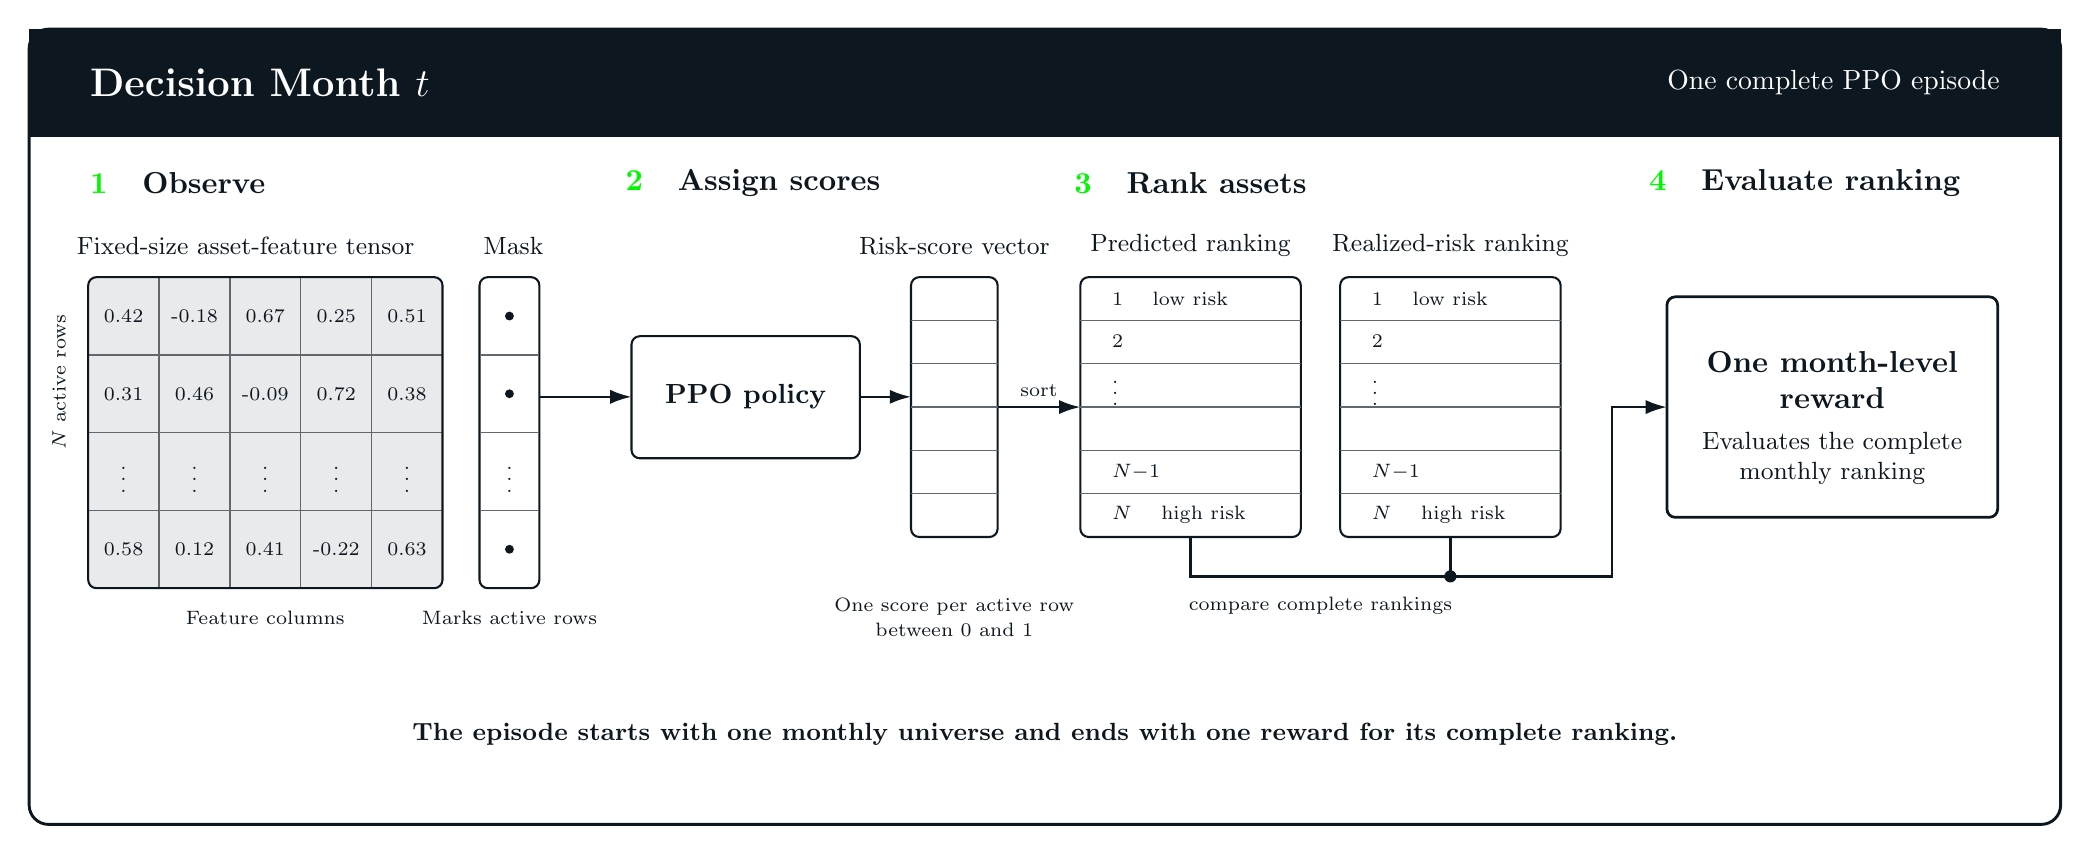
\begin{tikzpicture}[x=1cm,y=1cm]
  % Calendar-style episode boundary
  \draw[navy, line width=1.05pt, rounded corners=7pt] (0,0) rectangle (25.8,10.1);
  \draw[navy, line width=1.05pt] (0,8.75) -- (25.8,8.75);
  \fill[navy] (0,8.75) rectangle (25.8,10.1);
  \node[text=white, font=\bfseries\fontsize{14}{17}\selectfont, anchor=west]
    at (0.65,9.42) {Decision Month \(t\)};
  \node[text=white, font=\fontsize{10}{12}\selectfont, anchor=east]
    at (25.15,9.42) {One complete PPO episode};

  % Stage headings
  \node[stage, anchor=west] at (0.65,8.15) {\textcolor{green}{1}\quad Observe};
  \node[stage, anchor=west] at (7.45,8.15) {\textcolor{green}{2}\quad Assign scores};
  \node[stage, anchor=west] at (13.15,8.15) {\textcolor{green}{3}\quad Rank assets};
  \node[stage, anchor=west] at (20.45,8.15) {\textcolor{green}{4}\quad Evaluate ranking};

  % Observation: feature tensor
  \node[label] at (2.75,7.35) {Fixed-size asset-feature tensor};
  \fill[navy!9, rounded corners=3pt] (0.75,3.0) rectangle (5.25,6.95);
  \foreach \x in {1.65,2.55,3.45,4.35} {
    \draw[navy!65, line width=0.45pt] (\x,3.0) -- (\x,6.95);
  }
  \foreach \y in {3.9875,4.975,5.9625} {
    \draw[navy!65, line width=0.45pt] (0.75,\y) -- (5.25,\y);
  }
  \node[small] at (1.2,6.456) {0.42};
  \node[small] at (2.1,6.456) {-0.18};
  \node[small] at (3.0,6.456) {0.67};
  \node[small] at (3.9,6.456) {0.25};
  \node[small] at (4.8,6.456) {0.51};
  \node[small] at (1.2,5.469) {0.31};
  \node[small] at (2.1,5.469) {0.46};
  \node[small] at (3.0,5.469) {-0.09};
  \node[small] at (3.9,5.469) {0.72};
  \node[small] at (4.8,5.469) {0.38};
  \node[small] at (1.2,4.481) {\(\vdots\)};
  \node[small] at (2.1,4.481) {\(\vdots\)};
  \node[small] at (3.0,4.481) {\(\vdots\)};
  \node[small] at (3.9,4.481) {\(\vdots\)};
  \node[small] at (4.8,4.481) {\(\vdots\)};
  \node[small] at (1.2,3.494) {0.58};
  \node[small] at (2.1,3.494) {0.12};
  \node[small] at (3.0,3.494) {0.41};
  \node[small] at (3.9,3.494) {-0.22};
  \node[small] at (4.8,3.494) {0.63};
  \draw[outline] (0.75,3.0) rectangle (5.25,6.95);
  \node[small, rotate=90] at (0.38,5.62) {\(N\) active rows};
  \node[small] at (3.0,2.63) {Feature columns};

  % Mask strip
  \node[label] at (6.15,7.35) {Mask};
  \draw[outline] (5.72,3.0) rectangle (6.48,6.95);
  \foreach \y in {3.9875,4.975,5.9625} {
    \draw[navy!65, line width=0.45pt] (5.72,\y) -- (6.48,\y);
  }
  \fill[navy] (6.10,6.456) circle (1.6pt);
  \fill[navy] (6.10,5.469) circle (1.6pt);
  \node[small] at (6.10,4.481) {\(\vdots\)};
  \fill[navy] (6.10,3.494) circle (1.6pt);
  \node[small] at (6.1,2.63) {Marks active rows};

  % PPO black box and score vector
  \draw[outline] (7.65,4.65) rectangle (10.55,6.2);
  \node[text=navy, font=\bfseries\fontsize{10.2}{12.2}\selectfont, align=center]
    at (9.1,5.43) {PPO policy};
  \draw[arrow] (6.48,5.43) -- (7.65,5.43);

  \node[label] at (11.75,7.35) {Risk-score vector};
  \draw[outline] (11.2,3.65) rectangle (12.3,6.95);
  \foreach \y in {4.2,4.75,5.3,5.85,6.4} {
    \draw[navy!65, line width=0.45pt] (11.2,\y) -- (12.3,\y);
  }
  \node[small] at (11.75,2.63) {One score per active row\\between 0 and 1};
  \draw[arrow] (10.55,5.43) -- (11.2,5.43);

  % Predicted ranking
  \node[label] at (14.75,7.35) {Predicted ranking};
  \draw[outline] (13.35,3.65) rectangle (16.15,6.95);
  \foreach \y in {4.2,4.75,5.3,5.85,6.4} {
    \draw[navy!65, line width=0.45pt] (13.35,\y) -- (16.15,\y);
  }
  \node[small, anchor=west] at (13.63,6.68) {1 \quad low risk};
  \node[small, anchor=west] at (13.63,6.13) {2};
  \node[small, anchor=west] at (13.63,5.58) {\(\vdots\)};
  \node[small, anchor=west] at (13.63,4.48) {\(N{-}1\)};
  \node[small, anchor=west] at (13.63,3.93) {\(N\) \quad high risk};
  \draw[arrow] (12.3,5.3) -- node[small, above] {sort} (13.35,5.3);

  % Realized ranking
  \node[label] at (18.05,7.35) {Realized-risk ranking};
  \draw[outline] (16.65,3.65) rectangle (19.45,6.95);
  \foreach \y in {4.2,4.75,5.3,5.85,6.4} {
    \draw[navy!65, line width=0.45pt] (16.65,\y) -- (19.45,\y);
  }
  \node[small, anchor=west] at (16.93,6.68) {1 \quad low risk};
  \node[small, anchor=west] at (16.93,6.13) {2};
  \node[small, anchor=west] at (16.93,5.58) {\(\vdots\)};
  \node[small, anchor=west] at (16.93,4.48) {\(N{-}1\)};
  \node[small, anchor=west] at (16.93,3.93) {\(N\) \quad high risk};

  % Comparison and reward
  \draw[navy, line width=0.9pt] (14.75,3.65) -- (14.75,3.15) -- (18.05,3.15);
  \draw[navy, line width=0.9pt] (18.05,3.65) -- (18.05,3.15);
  \fill[navy] (18.05,3.15) circle (2.2pt);
  \node[small, below=4pt] at (16.4,3.15) {compare complete rankings};

  \draw[outline, line width=1pt] (20.8,3.9) rectangle (25.0,6.7);
  \node[text=navy, font=\bfseries\fontsize{11}{13}\selectfont, align=center]
    at (22.9,5.65) {One month-level\\reward};
  \node[label] at (22.9,4.65) {Evaluates the complete\\monthly ranking};
  \draw[arrow] (18.05,3.15) -- (20.1,3.15) -- (20.1,5.3) -- (20.8,5.3);

  % Bottom takeaway
  \node[text=navy, font=\bfseries\fontsize{9.5}{11.5}\selectfont, align=center]
    at (12.9,1.15)
    {The episode starts with one monthly universe and ends with one reward for its complete ranking.};
\end{tikzpicture}
\end{document}
